\algnewcommand{\LineComment}[1]{\State \(\triangleright\) #1}
% New definitions
\algnewcommand\algorithmicswitch{\textbf{switch}}
\algnewcommand\algorithmiccase{\textbf{case}}
\algnewcommand\algorithmicassert{\text{assert}}
\algnewcommand\Assert[1]{\State \algorithmicassert(#1)}%
% New "environments"
\algdef{SE}[SWITCH]{Switch}{EndSwitch}[1]{\algorithmicswitch\ #1\ \algorithmicdo}{\algorithmicend\ \algorithmicswitch}%
\algdef{SE}[CASE]{Case}{EndCase}[1]{\algorithmiccase\ #1}{\algorithmicend\ \algorithmiccase}%
\algtext*{EndSwitch}%
\algtext*{EndCase}%

\chapter{Simultaneous Multiple Quantile Estimation}
\label{ch: multi_quant}

\graphicspath{{Figures/Multi/}{./}} 

When the estimation for only a single quantile value is not enough, the idea of multi-quantile estimation appears. 
In this chapter we introduce the problem of simultaneous multi-quantile estimation along with two related methods. This chapter is organised as follow:

Section~\ref{sec: multi_intro} introduces the multi-quantile estimation for streaming data, followed by a discussion on the basic ideas to attack this problem. The next two sections will show how it is solved by methods focusing on different aspects.

Section~\ref{sec: multi_shiftQ} shows the \textit{shiftQ} algorithm for simultaneous quantile estimation by implementing the idea similar to SGD.

Section~\ref{sec: multi_{p2}} shows the \textit{$P^2$} algorithm that solves the problem in a much different way.

Section~\ref{sec: multi_discussion} list the comparison between the two methods, the discussion about the problem and our conclusion.

\section{The problem and opportunity of multi-quantile estimation}
\label{sec: multi_intro}

In real life implementations, quantile estimation usually do not focus on a single quantile value. For example, a common request is to show the median (the $0.5$-quantile) of the distribution, and at the same time show the outlier boundaries at ends of the distribution, like the $0.1$- and $0.9$- quantiles. It is also highly possible that more quantile estimates are required for the data distribution analysis.

Under this circumstance, the estimation of multiple different quantiles also 

% ----------------------------------- shiftQ ---------------------------------------
\iffalse

\section{The shiftQ methods}
\label{sec: multi_shiftQ}

\subsection{Method Description}

1. \textbf{Overall}: The basic idea is to estimate a central quantile point, and update other quantiles based on the central one. 

2. \textbf{Motivation}: The difference $diff$ between the two quantiles for the $x_{n}$ observation is:
$$
diff = |Q_x(q_{k+1}) - Q_x(q_k)|
$$
    Note that $diff > 0$ for all time, so different quantiles never cross each other. This property is guaranteed by the update function DUMIQE() and its restriction that the input quantile estimate must > 0.

3. \textbf{Update one quantile}: The difference is calculated based on the idea of "shift distribution". Let $X$ denotes the original distribution of data stream, and let distribution $Y$ denotes a shifted version of $X$ such that $Y = X + constant$. In this way, the quantile $q_{k+1}$ can be updated by implementation of shifting. The basic steps are:
\begin{itemize}
    \item Calculate $Q_x(q_k)$, which is the shift constant
    \item Get shift observation $y_{k+1} =  Q_x(q_k) - x$
    \item Calculate the new quantile $Q_y(q_{k+1})$ in $Y$
    \item Shift the change back to $X$: $Q_x(q_{k+1}) = Q_y(q_{k+1}) + shiftConstant$
\end{itemize}

4. \textbf{Update the bigger quantiles:} Starting from central quantile $q_c$, the estimates for $q_{c+1}, ..., q_{K}$ are calculated one based on another. So each time step 2 is repeated from $q_c$ to $q_{K-1}$

5. \textbf{Update the smaller quantiles:} Similar to step 3, for smaller quantiles, estimates for $q_{c-1}, ..., q_{1}$ are calculated similarly one based on another.

\subsection{The shiftQ Algorithm}
\begin{algorithm}
    \caption{The shiftQ Algorithm}\label{alg:multi_shiftQ}
        \begin{algorithmic}[1]
            \Require{Dataset $X$ (with positive data points only), Demanding quantile values $[\tau_1, \tau_2, ..., \tau_P]$}
            \Ensure{Demaning quantile estimates $[\tau_1\text{-}q, \tau_2\text{-}q, ..., \tau_P\text{-}q]$}
            % \Procedure{frugal}{$X,\tau$}            \Comment{X is the dataset}
            % \State {$d = 0, y_i = 0$ for $i = 1, 2, ..., n$}           \Comment{Default initialization}
            % \For{$k = 0,1,...$ \textbf{do}}                  %\Comment{Parameter update for each input data point}
            %     \State {Sample $i$ from {$1,2,...,n$}}
            %     \State {$d=d - y_i + f^{\prime}_i(x))$}
            %     \State {$y_i = f^{\prime}_i(x)$}
            %     \State{$x = x - \frac{\alpha}{n}d$}
            % \EndFor
            % \State{\textbf{end for}}
        \end{algorithmic}
\end{algorithm}
\subsection{Experiment Results}

\begin{figure*}[h!]
	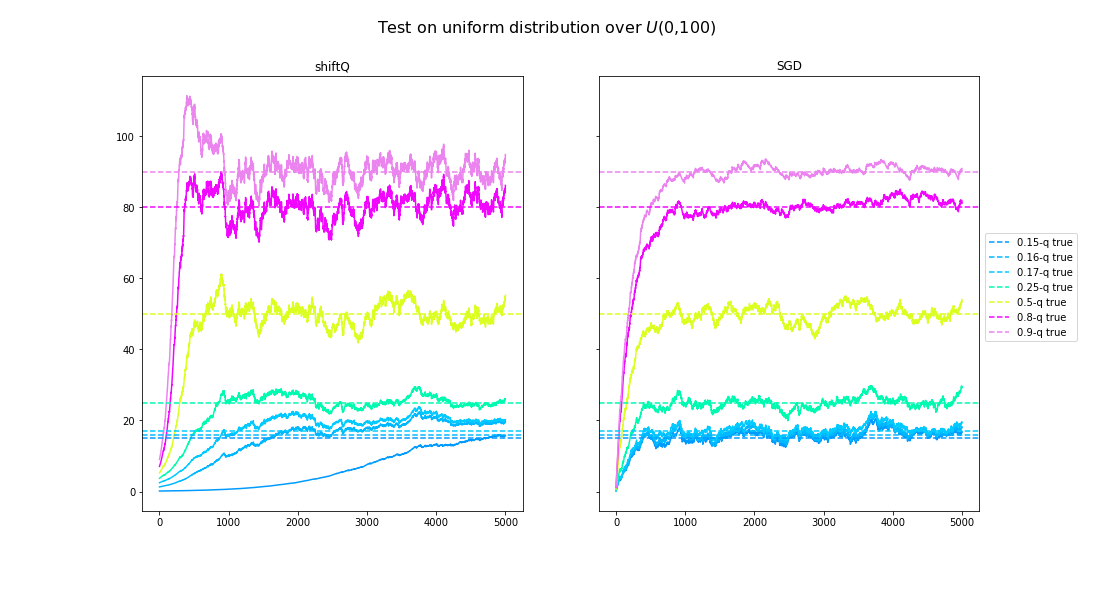
\includegraphics[width=1\columnwidth]{shiftQ/shiftQ_vs_SGD.png}
	\caption{Comparison between shiftQ and SGD}
\end{figure*}

\fi
% ----------------------------------- Extended P2 ---------------------------------------


\section{The Extended $P^2$ Algorithm}
\label{sec: multi_{p2}}

\subsection{Method Description}

\subsubsection{The $P^2$ Method}
\subsubsection{The Extended $P^2$ Method}

\subsection{The Algorithm of Extended $P^2$}

\section{Basic $P^2$ algorithm}

\begin{algorithm}
    \caption{$P^2$ Algorithm}\label{alg:multi_ext_p2}
        \begin{algorithmic}[1]
            \Require{Dataset $X$, Demanding quantile values $[\tau_1, \tau_2, ..., \tau_N]$}
            \Ensure{Demaning quantile estimates $[\tau_1\text{-}q, \tau_2\text{-}q, ..., \tau_N\text{-}q]$}
            \State
            \State{\textbf{A. Initialization}}
            \State {The first N observations (sorted): \{$x_1,x_2,...,x_N$\}}
            \For{$(i = 1, ..., N-1)$}
                \State {Marker height:    $q_i = x_i $}
                \State {Marker position:   $n_i = i$}
                \State {Desired Marker position:  $n_i\prime = (n-1)\tau_i + 1$}
            \EndFor

            \State
            \State{\textbf{B. For each new observation $x_j$, $j \geq N+1$, perform the following}}
            \LineComment {Find the cell $k$ such that $q_k \leq x_j < q_{k+1}$:}
            \Switch{$s$}
                \Case{$x_j < q_1$}
                    \State{$q_1 = x_j, k = 1$}
                \EndCase
                \Case{$q_i \leq x_j < q_{i+1}$}
                    \State {$k = i$}
                \EndCase
                \Case{$q_N < x_j$}
                    \State {$q_N = x_j, k = N-1$}
                \EndCase
            \EndSwitch
            \State
            \LineComment{Increment some marker positions:}
            \State{$n_i = n_i + 1$; $i = k+1, ..., N$}
            % \Comment{Different from that on the $P^2$ paper}
            \LineComment{Update all the desired positions:}
            \State{$n_i\prime = n_i\prime + \tau_i$}

            \State
            \LineComment{Adjust marker heights $2$ to $N-1$ if necessary:}
            \For{$i = 2, 3, ..., N-1$}
                \State {$d_i = n_i\prime - n_i$}
                \If {($ d_i \geq 1 \text{ and }  n_{i+1} - n_i > 1$) or 
                     ($ d_i \leq -1 \text{ and }  n_{i-1} - n_i < -1$) }
                    \State {$d_i = sign(d_i)$}
                    \State {$q_i\prime = P^2(q_1)$}     \Comment{Try the $P^2$ formula}
                    \If {$ q_{i-1} < q_i\prime < q_{i+1}$}
                        \State {$q_i = q_i\prime$}
                        \Else                           \Comment{Else use linear update}
                            \State{$q_i = \text{linear}(q_i)$}
                    \EndIf
                    \State {$n_i = n_i + d_i$}          \Comment{Update marker position}
                \EndIf
            \EndFor

            \State
            \State {\textbf{C. Return quantile estimates} }     
            \LineComment{The result is available after any number of observations}
            \State {$[\tau_1\text{-}q, \tau_2\text{-}q, ..., \tau_N\text{-}q] = [q_1, q_2, ..., q_N]$}
        \end{algorithmic}
\end{algorithm}

\subsection{Experiment Results}

% \begin{figure*}[h!]
% 	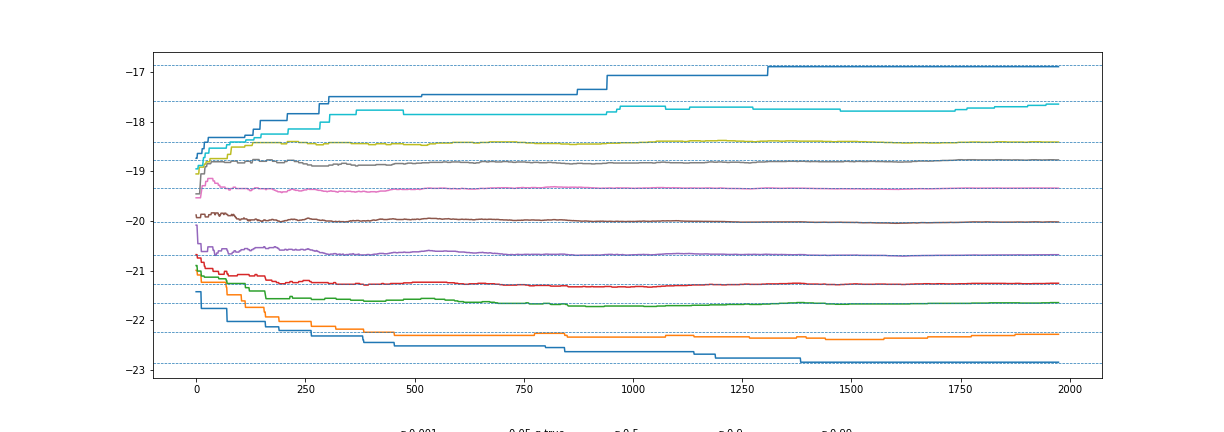
\includegraphics[width=1\columnwidth]{P2/P2.png}
% 	\caption{The P2 algorithm for Gaussian (mean = -20, std = 1)}
% \end{figure*}

% \begin{figure*}[h!]
% 	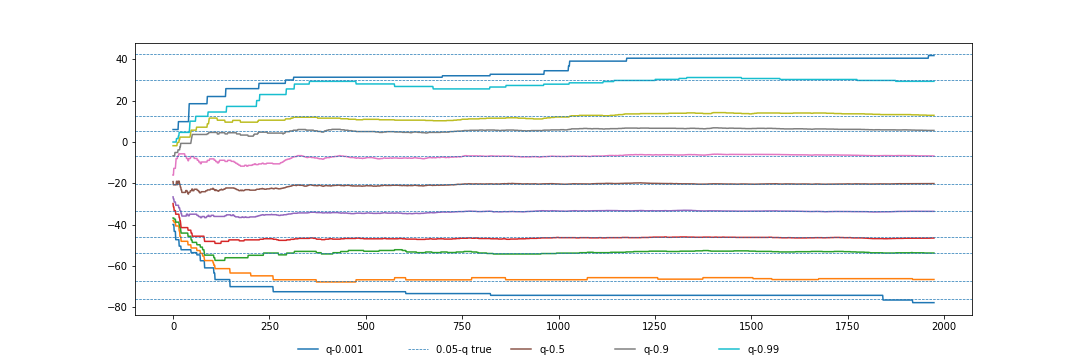
\includegraphics[width=1\columnwidth]{P2/P2_std_20.png}
% 	\caption{The P2 algorithm for Gaussian (mean = -20, std = 20)}
% \end{figure*}

% \begin{figure*}[h!]
% 	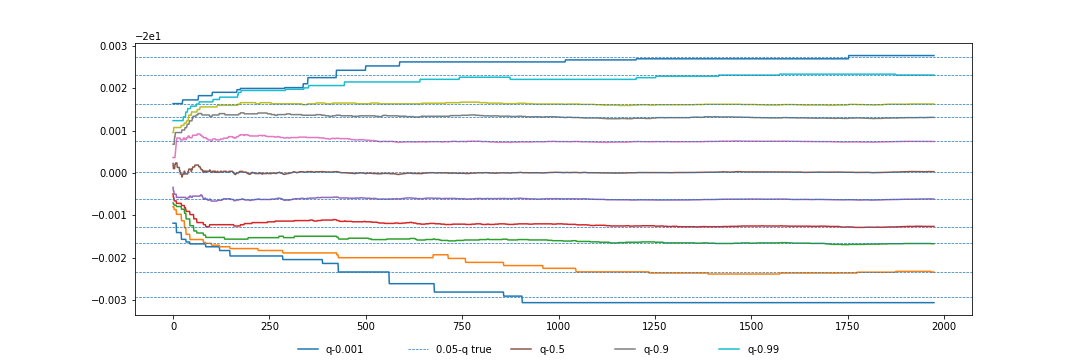
\includegraphics[width=1\columnwidth]{P2/P2_std_001.png}
% 	\caption{The P2 algorithm for Gaussian (mean = -20, std = $0.001$)}
% \end{figure*}

\section{Discussion and Conclusion}
\label{sec: multi_discussion}